%%%%%%%%%%%%%%%%%%%%%%%%%%%%%%%%%%%%%%%%%%%%%%%%%%%%%%%%%%%%%%%%%%%%%%
% How to use writeLaTeX: 
%
% You edit the source code here on the left, and the preview on the
% right shows you the result within a few seconds.
%
% Bookmark this page and share the URL with your co-authors. They can
% edit at the same time!
%
% You can upload figures, bibliographies, custom classes and
% styles using the files menu.
%
%%%%%%%%%%%%%%%%%%%%%%%%%%%%%%%%%%%%%%%%%%%%%%%%%%%%%%%%%%%%%%%%%%%%%%

\documentclass[12pt]{article}

\usepackage{sbc-template}

\usepackage{graphicx,url}

%\usepackage[brazil]{babel}   
\usepackage[utf8]{inputenc}  

     
\sloppy

\title{Método de Data Mining aplicado para predição de Diabetes Mellitus}

\author{\\Alexander B. Reis\inst{1}\\Arthur H. R. Teixeira\inst{2}\\Bernardo M. Alfredo\inst{3}\\Marcos T. M. Rezende\inst{4}\\Pedro D. Aguiar\inst{5}}


\address{Instituto de Ciências Exatas e Informática -- Pontifícia Universidade\\
Católica de Minas Gerais (PUC-MG)\\
Tópicos I\\
Orientador: Luis E. Z. Galvez
\email{alexander.reis@sga.pucminas.br\inst{1}, ahrteixeira@sga.pucminas.br\inst{2},}
\email{bernardo.alfredo@sga.pucminas.br\inst{3}, mtmrezende@sga.pucminas.br\inst{4},}
\email{pdaguiar@sga.pucminas.br\inst{5}}
}

\begin{document}

\maketitle
     
\begin{resumo}

  Caracterizando o perfil de Diabetes Millitus, realizamos um estudo e experimento de Data Mining para elaborar um classificador para predição de casos de Diabetes. Utilizando de uma base de dados de 2013, tratando-a e cultivando os atributos relevantes para a doença e gerando um classificador, por meio do algoritmo de Random Forest.
  
\end{resumo}

\section{Introdução}

Cientificamente conhecida como Diabetes Mellitus, a Diabetes é uma doença metabólica crônica caracterizada pelo aumento dos níveis de açúcar/glicose no sangue. Causada pela insuficiência ou mau funcionamento da insulina (hormônio que transporta a glicose do sangue para as células), resultando no acúmulo de açúcar no sangue ao invés de ser gasto nas células do corpo.\\\\
A Organização Mundial de Saúde (OMS) afirma que em torno de 422 milhões de adultos estão com diabetes no mundo, já no Brasil, segundo o IBGE, temos 9 milhões de brasileiros com diabetes, ou mais de 6\% da população.\\\\
Tivemos como objetivo, portanto, a predição da Diabetes Mellitus com base nas características apresentadas pelo indivíduo. Para isso, utilizamos da Analise de Dados, através das ferramentas: Python (Blibliotecas Pandas, Sklearn, entre outros), Weka, Excel.\\\\
Percebemos que como a quantidade de casos de Diabetes no Brasil e no mundo é grande, vemos uma possibilidade de trabalhar em uma base de dados para analisar o indivíduo e predizer se o mesmo tem a doença ou se seu quadro é relacionado como alguém que possua a doença, para que os diagnósticos possam ser feitos de maneiras mais simplificadas e ágeis.\\\\
Podemos destacar entre os artigos base o \textit{Performance Analysis of Classifier Models to Predict Diabetes Mellitus} \cite{KANDHASAMY201545} e o \textit{Machine Learning and Data Mining Methods in Diabetes Research} \cite{KAVAKIOTIS2017104}, no qual eles trabalharam com os métodos e algoritmos de Data Mining para auxílio na predição de casos de Diabetes Millitus. Um deles discorre sobre a performance e eficiência dos algoritmos de Machine Learning e o outro aborda os pontos fortes do uso dessa ferramenta para a realização de diagnósticos e classificações em pacientes iniciais.\\\\
Como nosso objetivo é a predição da Diabetes através das ferramentas de Data Mining e Machine Learning, pudemos explorar uma parte desse assunto, aprofundando as análises e simulações que estes trabalhos anteriores realizaram.\\\\
Este trabalho está dividido em 4 seções. A primeira seção trata sobre os trabalhos relacionados, discorrendo um pouco sobre as propostas e resultados que os autores obtiveram. Na segunda seção abordaremos os metodologia que utilizamos para o desenvolvimento do nosso trabalho, tais como materiais e métodos aplicados. A terceira seção descreve o desenvolvimento experimental de nosso trabalho, além da análise dos resultados obtidos. E por fim, na quarta seção apresentamos nossa conclusão e sugestão para trabalhos futuros.

\section{Trabalhos Relacionados}
No artigo \textit{Performance Analysis of Classifier Models to Predict Diabetes Mellitus} \cite{KANDHASAMY201545} os autores comparam o desempenho dos algoritmos mais usados para prever o diabetes usando técnicas de Data Mining. Nesse artigo é apresentado comparações dos classificadores de aprendizado de máquina (Árvore de Decisão J48, KNN, Random Forest e SVM) para classificar pacientes com Diabetes Mellitus. Foi usado amostras de dados baixadas do repositório de dados de aprendizado de máquina UCI. O desempenho dos algoritmos foi medido em ambos os casos, ou seja, antes do pré-processamento e após o pré-processamento, e comparados em termos de precisão, sensibilidade e especificidade.\\
No cenário de pré-processamento do conjunto de dadosos estudos e testes concluíram que o classificador da Árvore de Decisão J48 atinge maior precisão de 73,82\% do que os outros três classificadores. Mas, após o pré-processamento do conjunto de dados, o KNN e Random Forest têm um desempenho muito melhor do que os outros três classificadores e fornecem alta precisão. A partir disso, podemo-nos basear nossa escolha do algoritmo de classificação que usamos no nosso trabalho (Random Forest).\\\\
Já no artigo \textit{Machine Learning and Data Mining Methods in Diabetes Research} \cite{KAVAKIOTIS2017104} os autores tiveram como objetivo realizar uma revisão sistemática de aplicações de Machine Learning, técnicas de Data Mining e ferramentas no campo da pesquisa do Diabetes, com a finalidade de abordar predição e diagnóstico, complicações diabéticas, antecedentes genéticos e meio ambiente, e assistência e gestão em saúde.\\
Nesse estudo, um esforço sistemático foi feito para identificar e revisar aprendizado de máquina e abordagens de Data Mining aplicadas na pesquisa de Diabetes Mellitus. O advento da biotecnologia, com a vasta quantidade de dados produzidos, espera-se que dê origem a uma exploração mais aprofundada para o diagnóstico, etiopatofisiologia e tratamento de Diabetes através do emprego de técnicas de aprendizagem de máquina e Data Mining em conjuntos de dados enriquecidos que incluem informações clínicas e biológicas.

\section{Metodologia}

Apresentaremos como  desenvolvemos nosso trabalho, os materiais e métodos usados e adotados.

\subsection{Materiais}

Foi utilizada a base de dados obtida a partir da Pesquisa Nacional de Saúde 2013, realizada pelo IBGE. Para o problema em questão, a base de dados foi tratada, sendo mantidos os atributos relevantes para o problema da Diabetes.

\subsection{Métodos}

Elaboramos um Modelo Conceitual, representado pela Figura \ref{fig:diabetes_concept_map} abaixo:

\begin{figure}[h]
    \centering
    \caption{Modelo Conceitual Diabetes}
    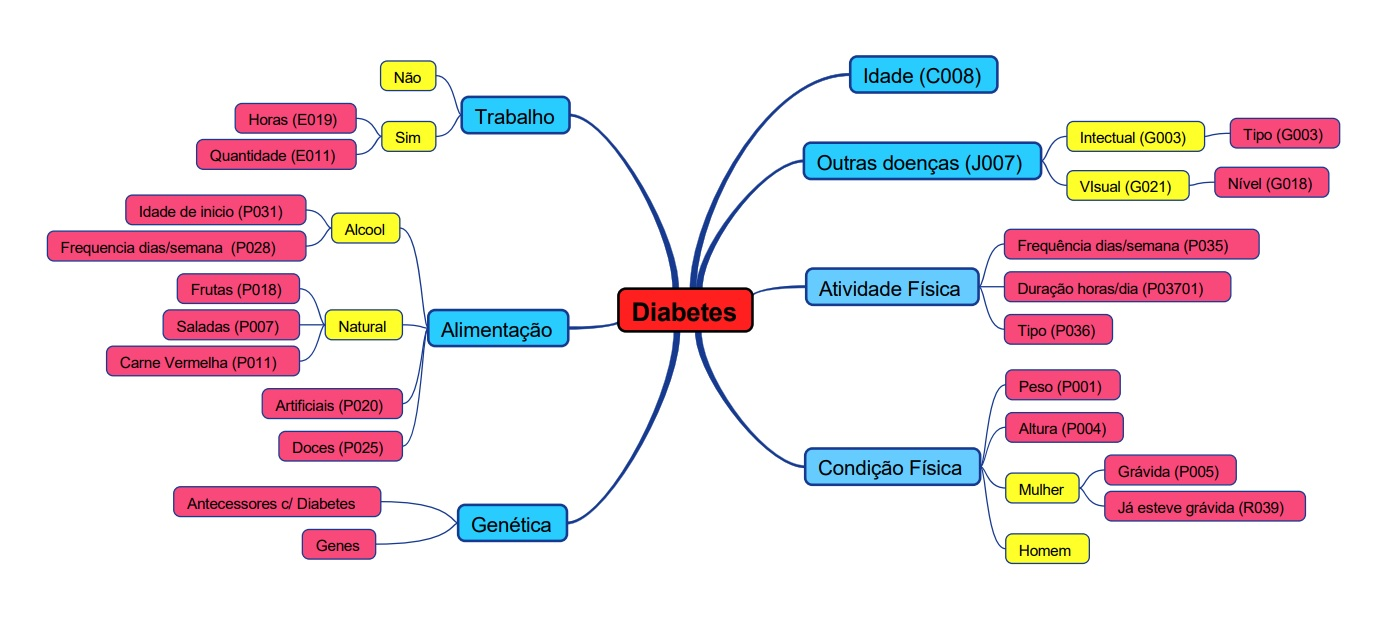
\includegraphics[scale=0.38]{Diabetes_Concept_Map.jpg}\\
    {\footnotesize Fonte: Elaborada pelos autores.}
    \label{fig:diabetes_concept_map}
\end{figure}
\\
Por orientação, verificamos se havia a necessidade de focar em algum estado do país, o que não foi necessário, uma vez que todos estados são balanceados.\\\\
Ao analisarmos o atributo Q30 – Diagnostico de diabetes, podemos ver que a base se encontra perfeitamente balanceada, não sendo necessária nenhuma ação quanto a isso.\\

\begin{figure}[!htb]
    \centering
    \caption{Pré-Processamento – Balanceamento}
    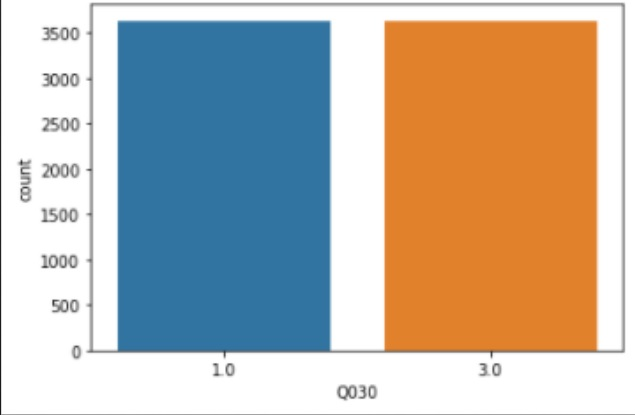
\includegraphics[scale=0.65]{Pre_processamento_balanceamento.jpg}\\
    {\footnotesize Fonte: Elaborada pelos autores.}
    \label{fig:pre_processamento_balanceamento}
\end{figure}

\newpage Inicialmente haviam 972 atributos. A partir de pesquisas sobre o problema, reduzimos essa quantidade para 18. Com auxilio de um profissional da área da saúde, aumentamos esse número para 32. Analisamos possíveis atributos de causa e dependências entre atributos. Finalizando com o total de 23 atributos.\\\\
Utilizamos o método \textit{.isna()}, do Pandas, para avaliar os atributos com dados ausentes e o método \textit{.fillna()}, também do Pandas, com o parâmetro ‘moda’, para substituir os dados ausentes pela moda do atributo. Assim, não alterando o média do atributo.\\\\
Identificamos os atributos contínuos. Utilizamos do gráfico de dispersão para verificação. Com exceção do atributo idade, todos apresentaram outliers porém, com dados dentro da realidade. Decidimos por manter os registros com outliers, pois poderiam ser de importância para os resultados. Os atributos contínuos são: Idade, Peso Aproximado, Doses de bebida por semana, Idade que iniciou a beber.

\begin{figure}[h]
    \centering
    \caption{Outliers - Peso Aproximado}
    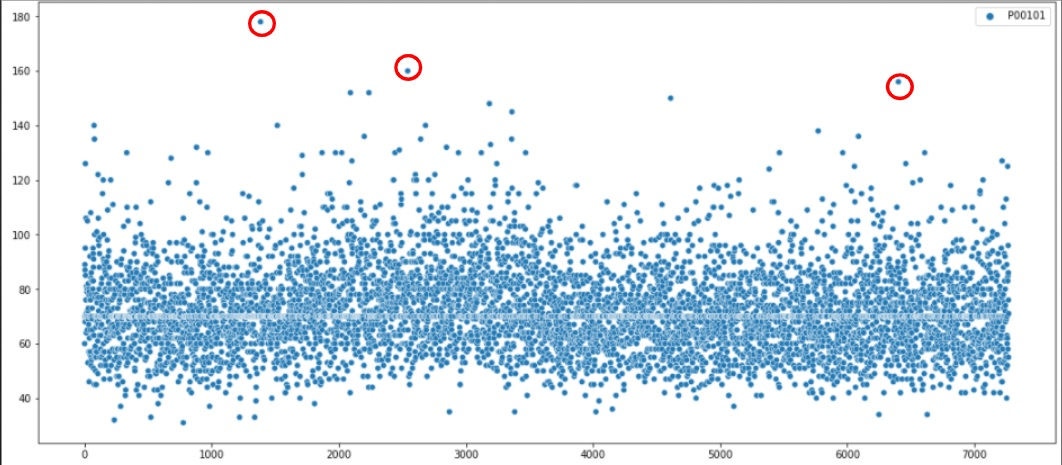
\includegraphics[scale=0.45]{Outliers_peso_aproximado.jpg}\\
    {\footnotesize Fonte: Elaborada pelos autores.}
    \label{fig:outliers_peso_aproximado}
\end{figure}

\begin{figure}[h]
    \centering
    \caption{Outliers - Doses de Bebida por Semana}
    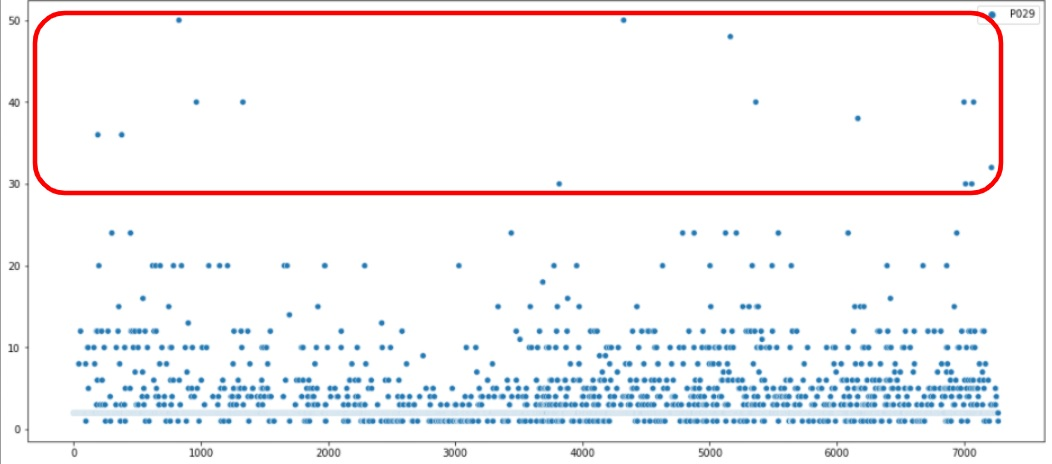
\includegraphics[scale=0.45]{Outliers_doses_bebida_semana.jpg}\\
    {\footnotesize Fonte: Elaborada pelos autores.}
    \label{fig:outliers_doses_bebidas_semana}
\end{figure}

Utilizamos o algoritmo \textit{Discretize} no software Weka. A discretização é feita por binning simples. Alteramos os parâmetros (os demais permaneceram no valor padrão):\\\\
- \textit{ignoreClass}: true, para ignorar o atributo de classificação.\\
- \textit{findNumBins}: true, para otimizar o número de caixas de largura igual.

\subsection{Desenvolvimento Experimental e Análise de Resultados}

Utilizamos o algoritmo Random Forest para a classificação da base. A base foi divida em 70\% para treino e 30\% para testes. Obtivemos os seguintes resultados:\\\\
- Coeficiente de Correlação: 0.5311\\
- Erro Médio Absoluto: 0.7503\\
- Raiz Quadrada Média do Erro: 0.8495\\
- Erro Absoluto Relativo: 75.0327 \%\\
- Raiz Quadrada do Erro Relativo: 84.9453 \%\\
- Número Total de Instâncias: 2182\\\\
A porcentagem de erro foi grande no nosso experimento, tentamos excutar o algoritmo outras vezes, mas a média do erro permanecia a mesma, cerca de 75\%.

\section{Conclusões e Trabalhos Futuros}

Mesmo executando os passos propostos pela disciplina, no final do experimento não conseguimos uma boa eficiência no desempenho do classificador, o que nos deixa uma questionamento, a quantidade de processos aplicados na base de dados foi baixa, ou as entradas dos dados e, juntamente, com a ocorrência de dados ausentes influênciaram para a margem de erro subir bastante. Temos, portanto, sugestão para trabalhos futuros, os quais possam explorar esse ponto de vista, realizando experimentos com a base de dados sem estar totalmente tratada, analisar os dados ausentes, e talvez, utilizar outro tipo de algoritmo para gerar o classificador.

\bibliographystyle{sbc}
\bibliography{sbc-template}

\end{document}
